\justify
{
\index{Definition of data structure}{\huge\textcolor{red}{\hspace{5 mm}D}}ata structure is a special way of organizing data in a computer so that we can use those efficiently later. Types of data structures means how the data structure implemented and how it looks like when comparing with the real world, how structured the skeleton that stayed beyond of that data structure, is it linear or non-linear? is it stack type or hierarchical tree type as well.\\
\index{Basic types of data-structure}The two basic types of data-structure:
\begin{enumerate}
	\item Linear
	\item Non-linear
\end{enumerate}
\index{Algorithmic notations}
To solve a problem we builds some different logic and algorithm but we don't know actually which algorithm is more efficient for our program in terms of holding less memory and shortest time. That's why we compare algorithms in a manner to find out best algorithmic approach that takes less memory and shortest time to make our program efficient. Due to respect of finding best algorithm there are so many approaches and they are denoted by some kind of mathematical notations. By those notations we measure the performance of an algorithm and scalability.\\
Some notations are:
\begin{enumerate}
	\item Big Theta notation $\theta(\textrm{ })$
	\item Big Ow notation $O(\textrm{ })$
	\item Big Omega notation $\omega(\textrm{ })$
\end{enumerate}
\index{Analysis graph by BIG O notation} Mostly used notation here is big Ow notation $O(\textrm{ })$. Here is a complexity analysis graph via big Ow notation $O(\textrm{ })$.
}
	\begin{figure}[h!]
	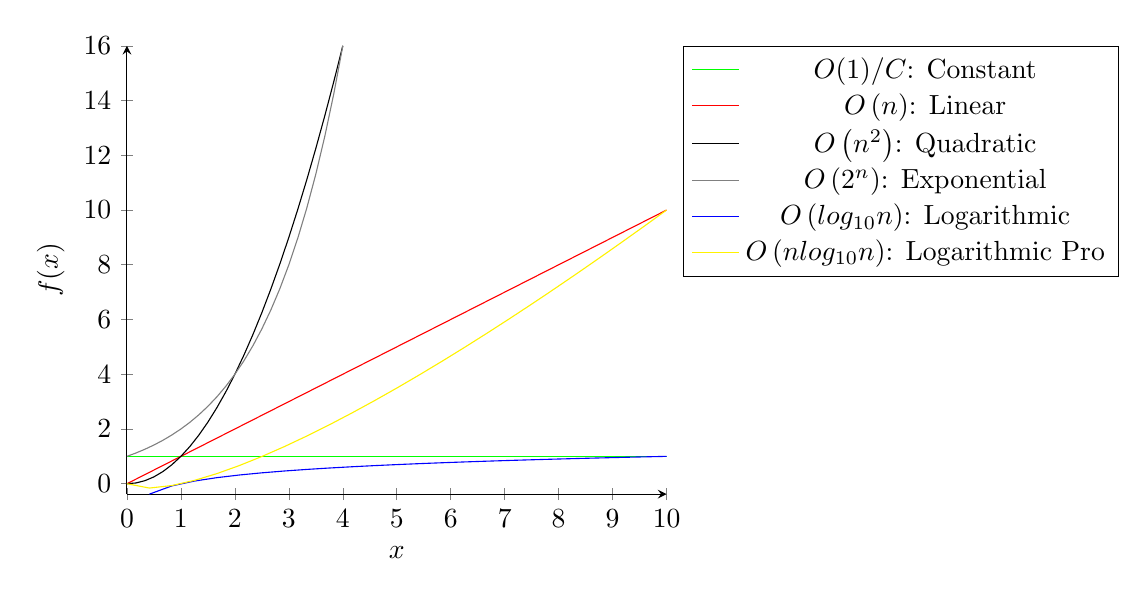
\begin{tikzpicture}
	
		\begin{axis} [
						axis lines = left,
						xlabel = $x$,
						ylabel = $f(x)$,
						legend pos = outer north east,
						xtick = {0, 1, 2,...,10},
						ytick = {0, 2,...,16}
					 ]
			\addplot[green, domain = 0:10] {1};
			\addplot[red, domain = 0:10] {x};
			\addplot[black, domain = 0:4] {x^2};
			\addplot[gray, domain = 0:4] {2^x};
			\addplot[blue, domain = 0:10] {log10(x)};
			\addplot[yellow, domain = 0:10] {x*log10(x)};
			
			\legend{$O(1) / C$: Constant, $O\left(n\right)$: Linear, $O\left(n^2\right)$: Quadratic, $O\left(2^n\right)$: Exponential, $O\left(log_{10}n\right)$: Logarithmic, $O\left(nlog_{10}n\right)$: Logarithmic Pro}
		\end{axis}
		
	\end{tikzpicture}
	\centering
	\caption{Complexity analysis graph due to respect of BIG $O$}
	\end{figure}